\chapter{Original borehole log sheets}
\label{chapter:Borehole_logsheets}

In the first half of the year 2016 Conservation Alliance (CA) commissioned the construction of multiple boreholes in northern Ghana. The boreholes subjected in this research (five locations, visualized in \ref{fig:Overviewlocations})are all part of this operation. Valuable information is gained with respect to local soil stratification, during borehole construction. Information is preserved in the original borehole log-sheets, which can be found in this appendix. Besides the local soil stratification, these log-sheets contain information on individual applied well structures. A depth dependent distinction is made in plain versus screened well skin. In terms of content these borehole log-sheets are used as a starting point in the theoretical model determination (section \ref{section:derivation_methods}). 

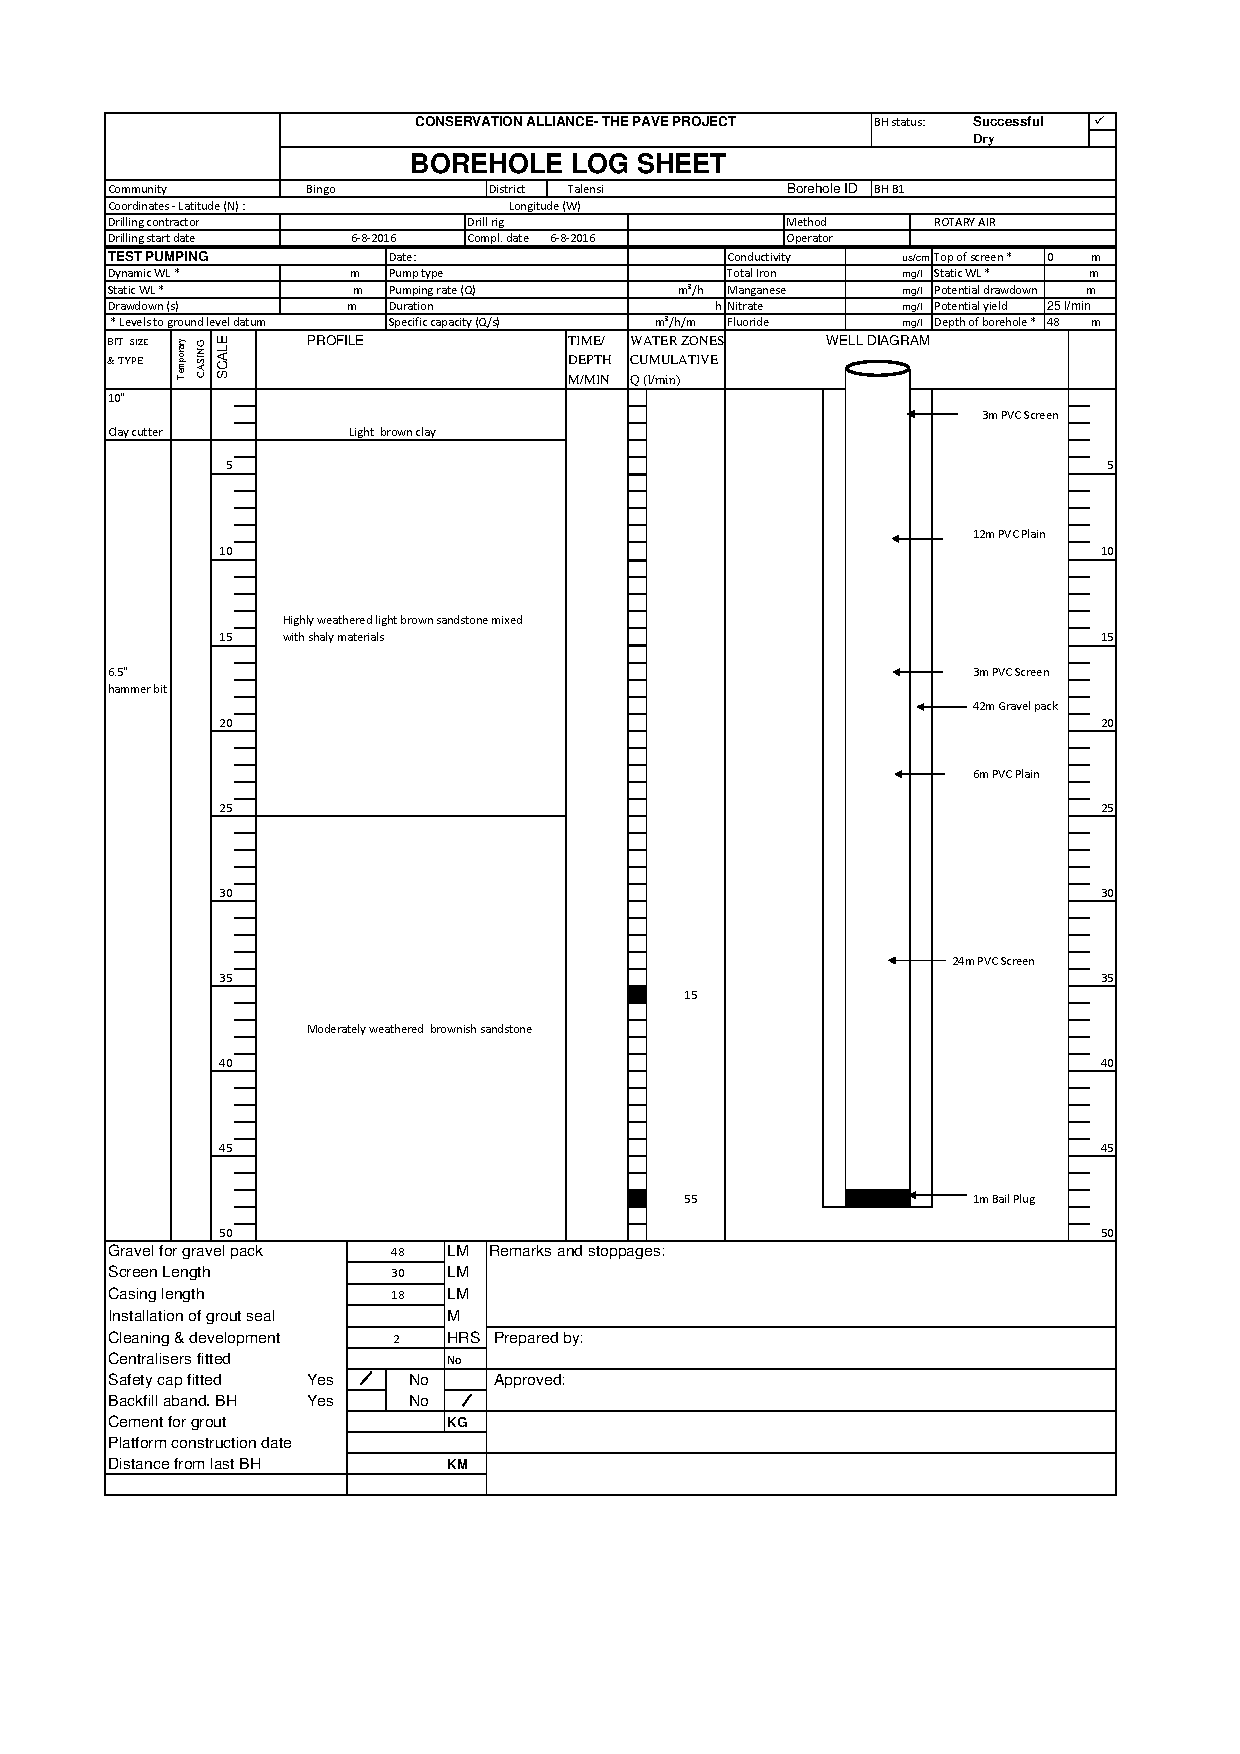
\includepdf[pages={1}]{BH_Bingo.pdf}
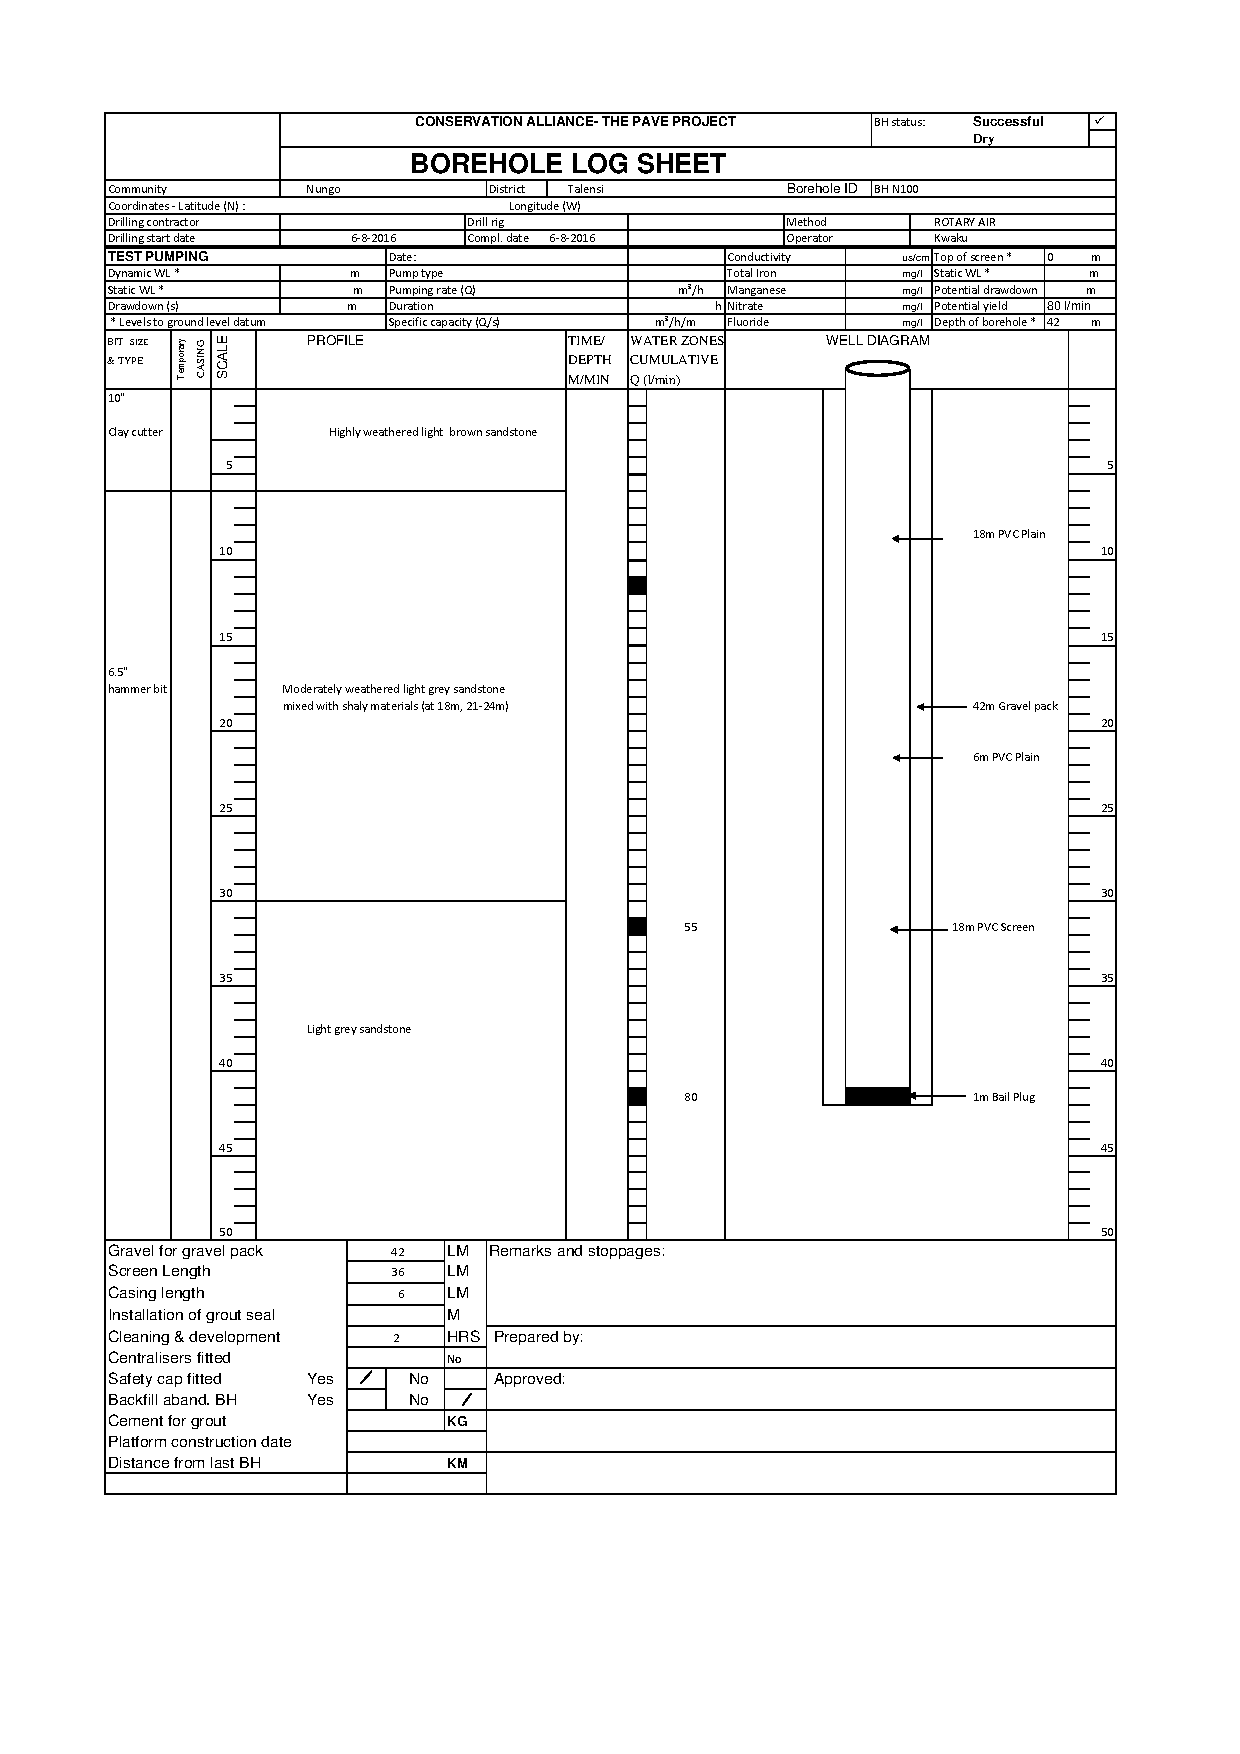
\includepdf[pages={1}]{BH_Nungo.pdf}
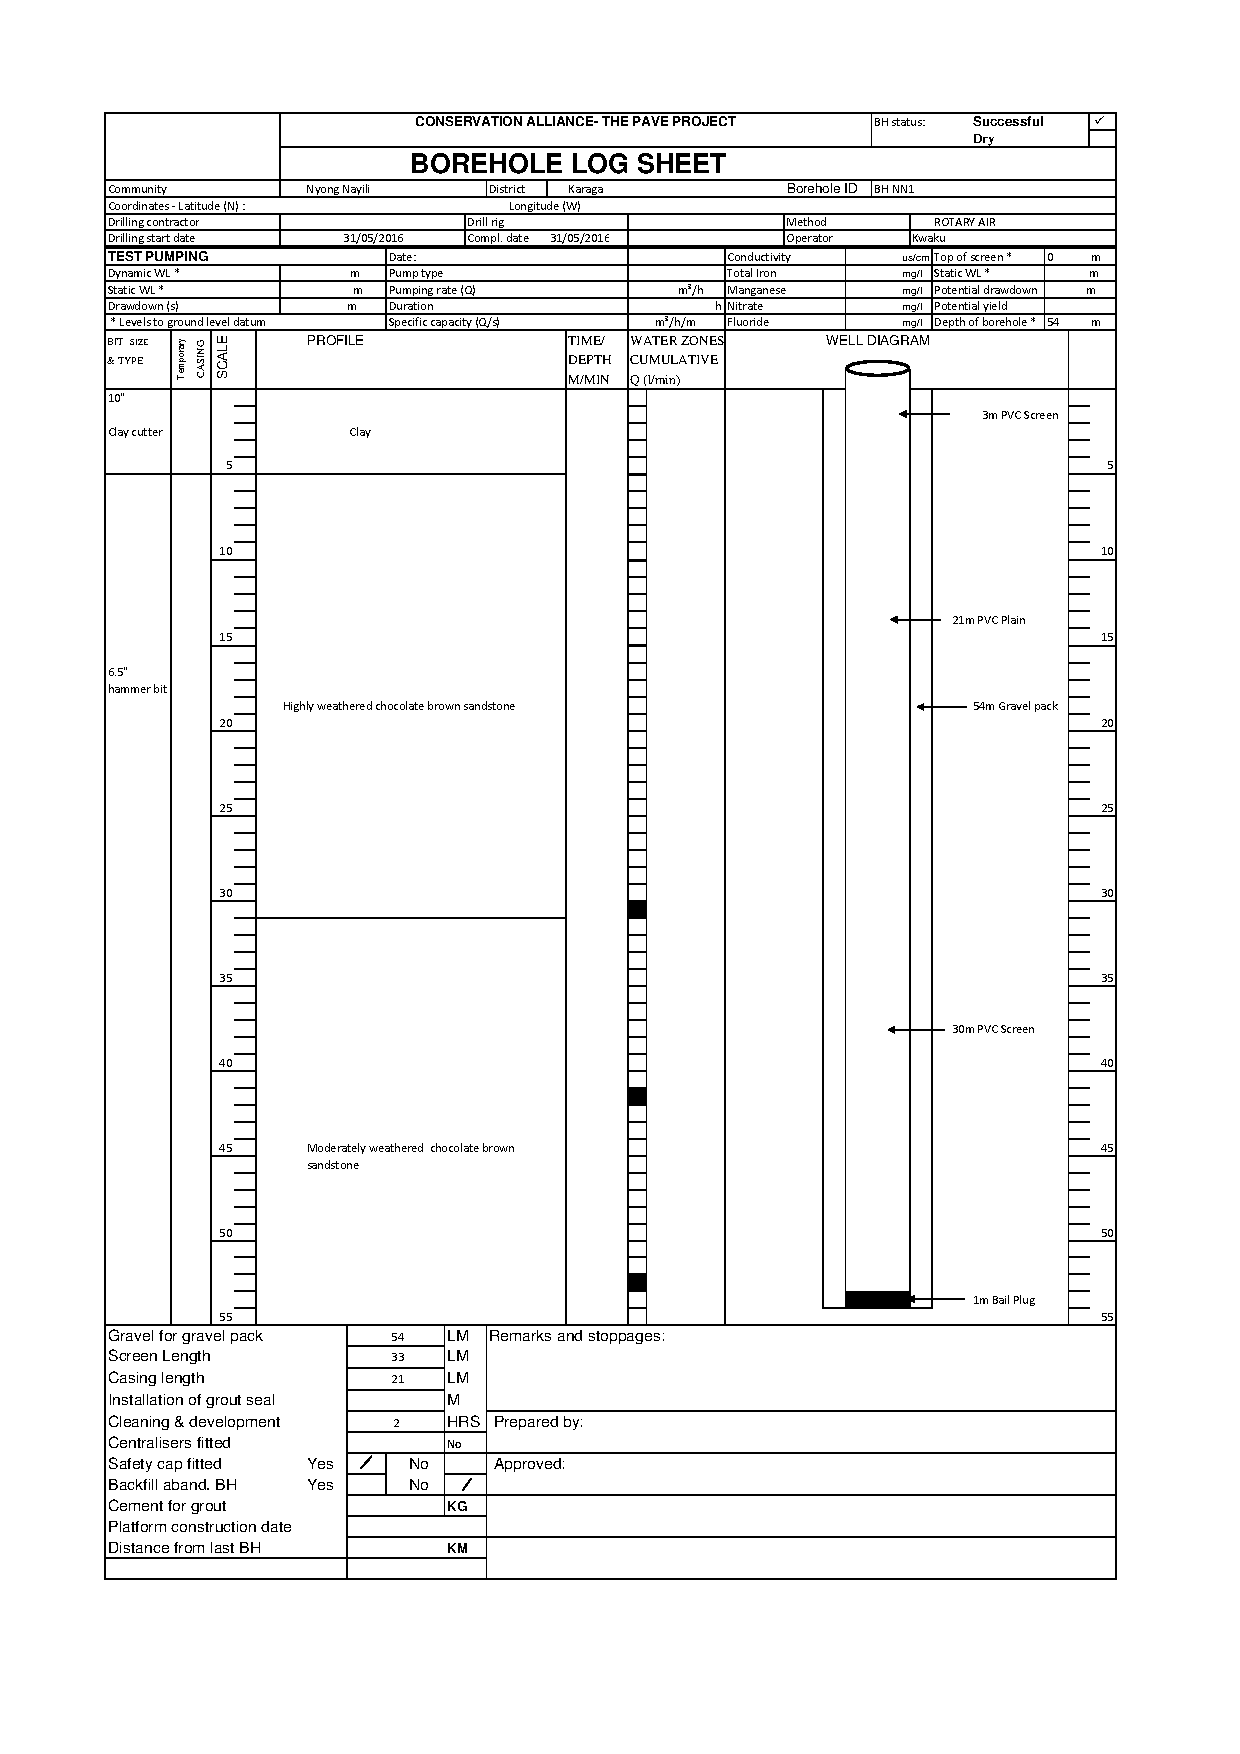
\includepdf[pages={1}]{BH_Nyong_Nayili.pdf}
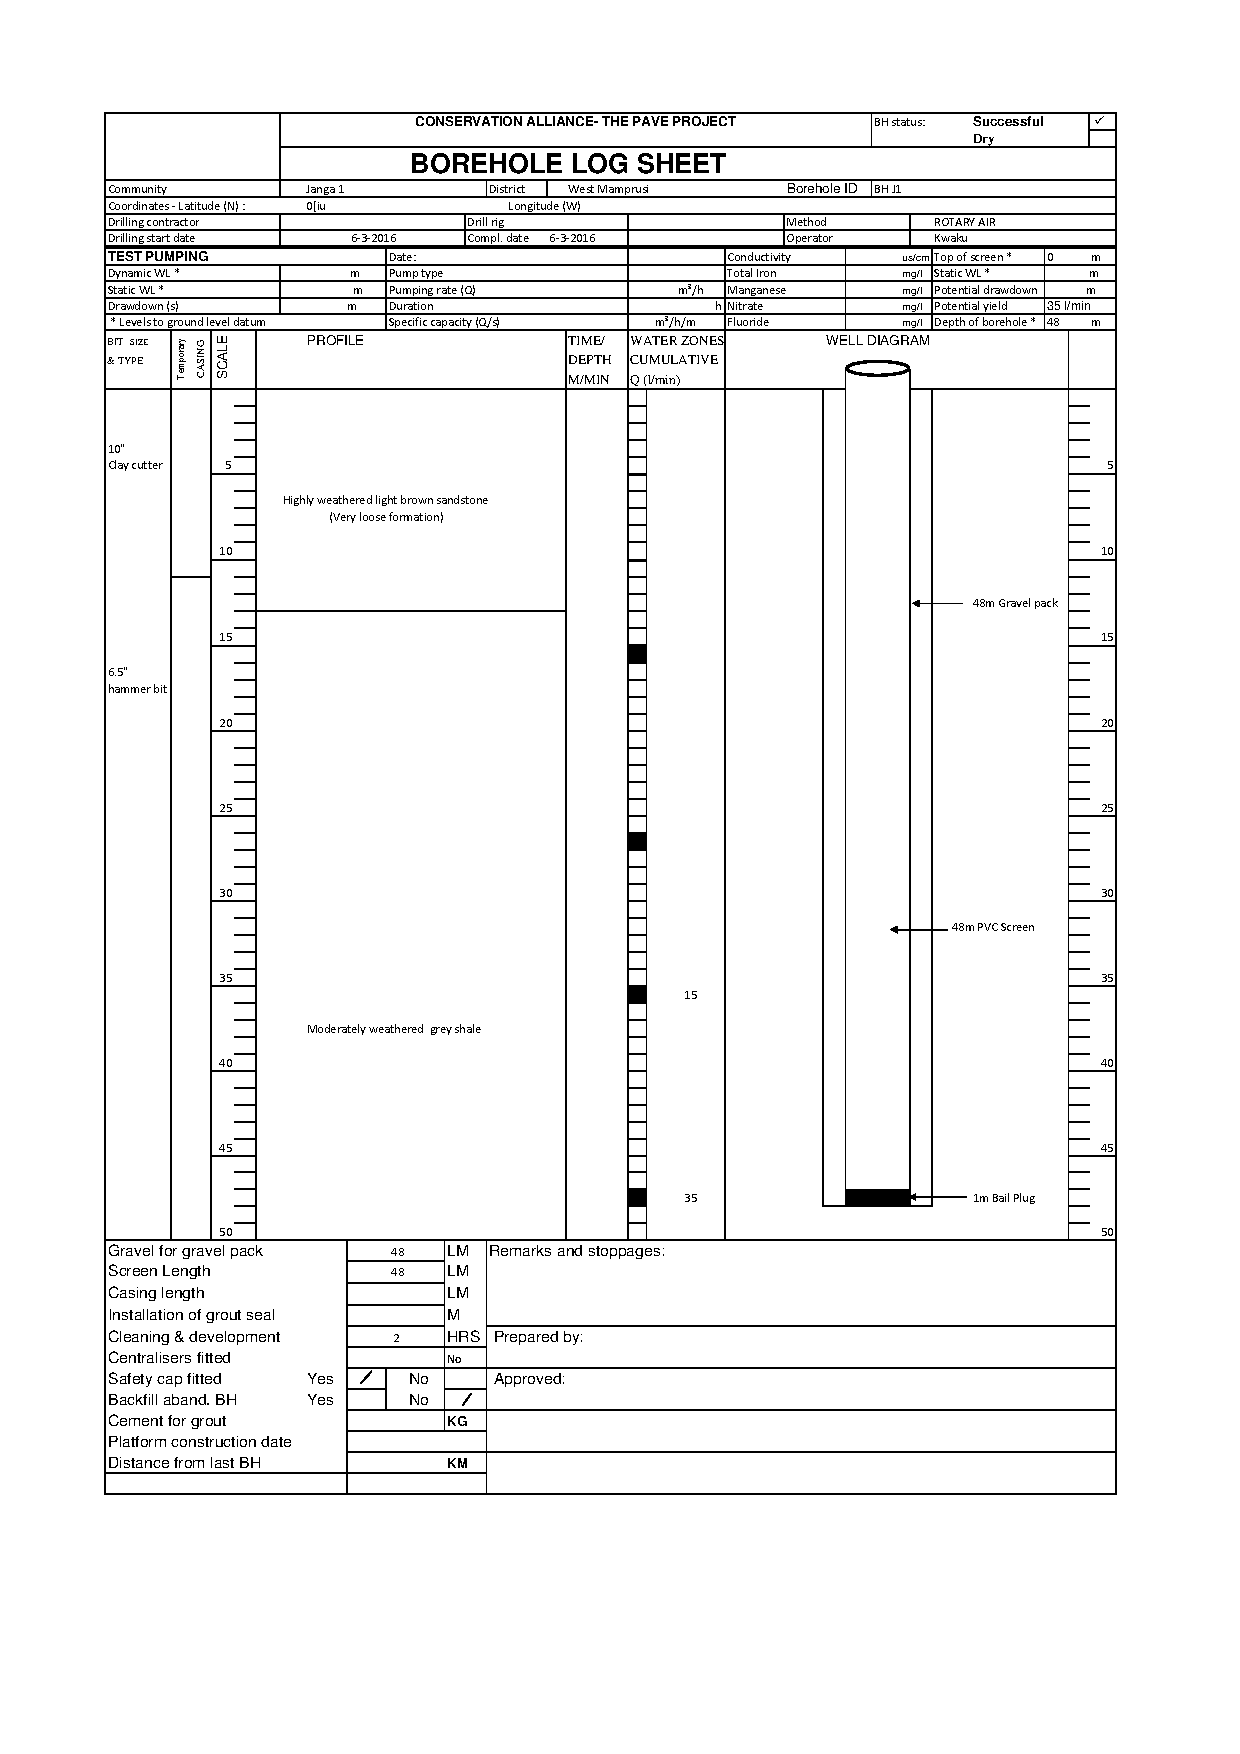
\includepdf[pages={1}]{BH_Janga.pdf}
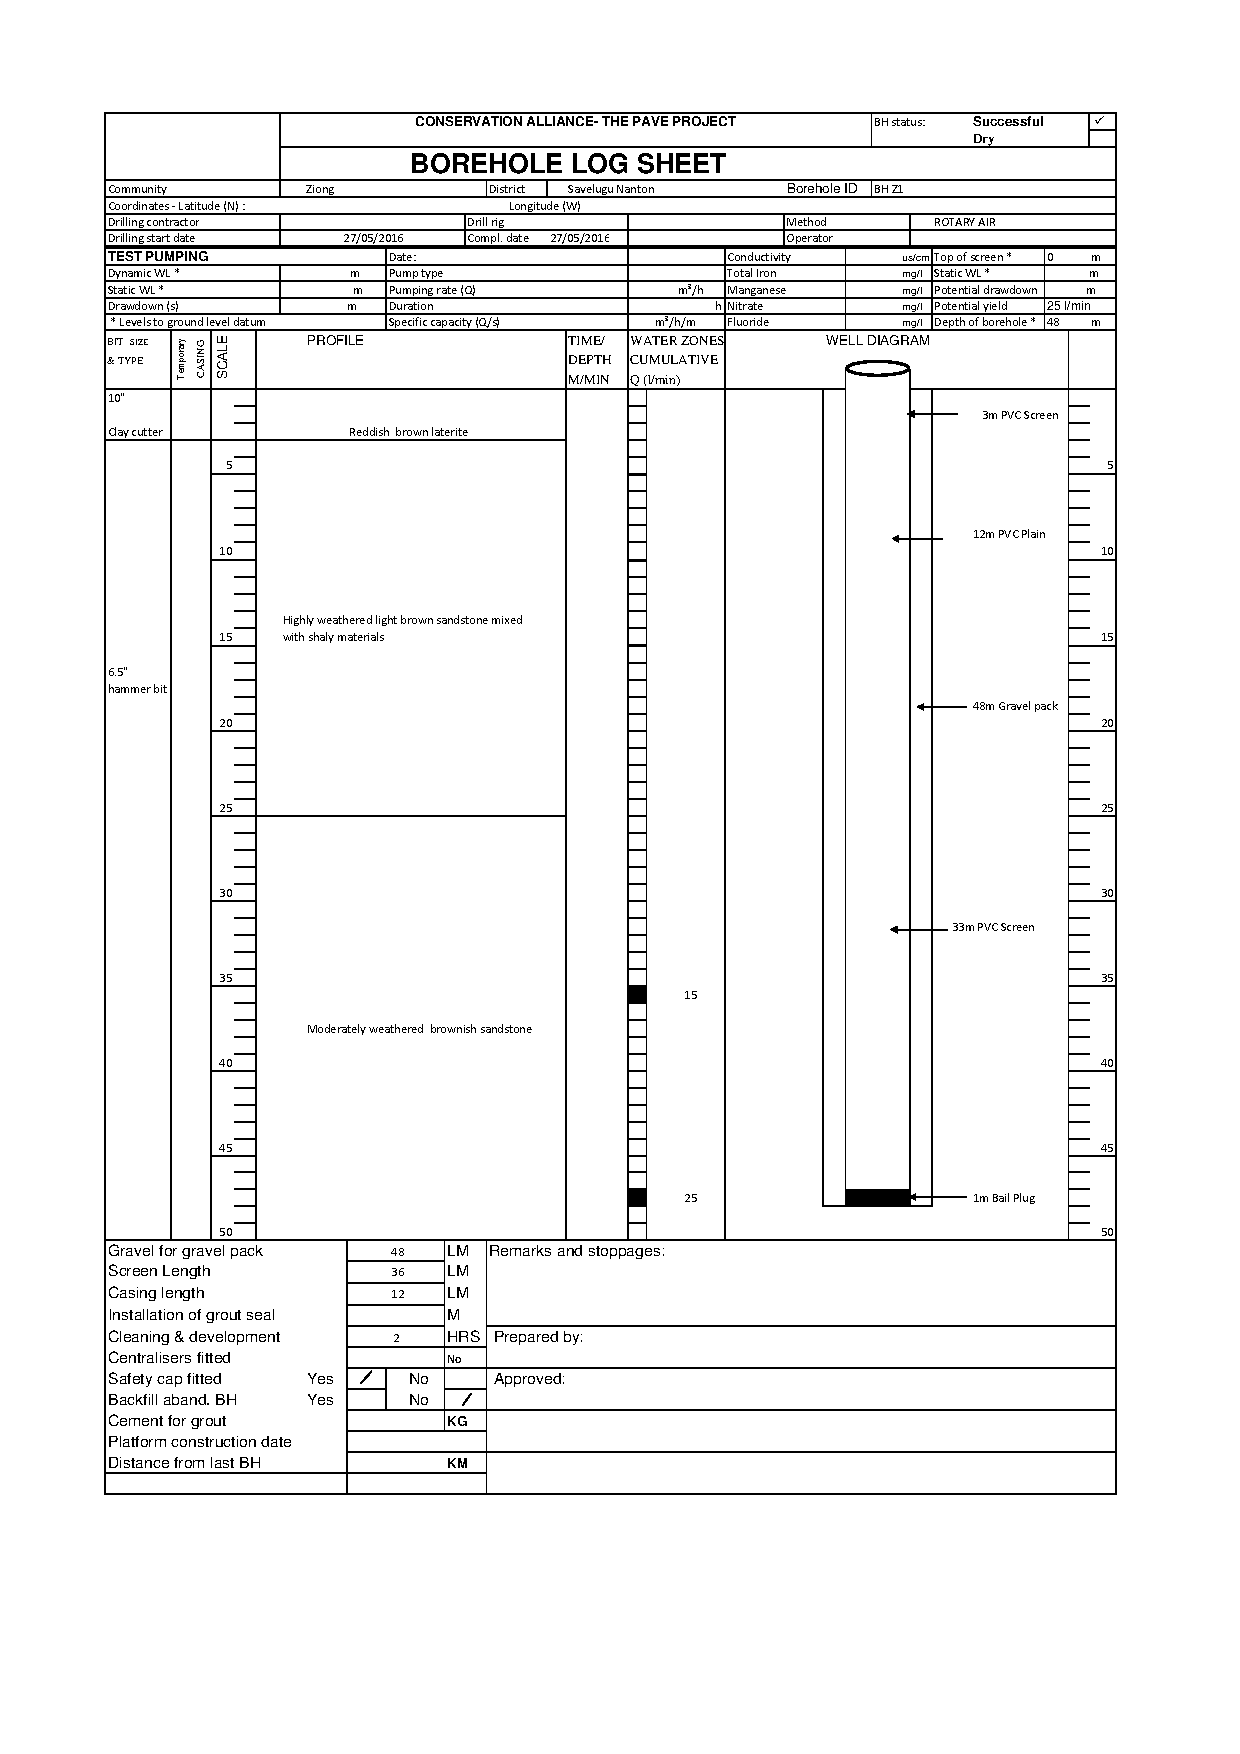
\includepdf[pages={1}]{BH_Ziong.pdf}